\chapter{Установка и настройка Seafile}
\label{ch:practice}

\section{Установка зависимостей}

\subsection{Python и системные пакеты}

\begin{lstlisting}
apt-get update
apt install python3 python3-setuptools python3-pip libmysqlclient-dev
\end{lstlisting}

Установка Python-пакетов через pip:
\begin{lstlisting}
pip3 install --timeout=3600 django==3.2.* Pillow pylibmc captcha jinja2 \\
  sqlalchemy==1.4.3 django-pylibmc django-simple-captcha python3-ldap \\
  mysqlclient pycryptodome==3.12.0 cffi==1.14.0
\end{lstlisting}

\subsection{MariaDB}

\begin{lstlisting}
apt install mariadb-server
\end{lstlisting}

Устанавливаем пароль root MariaDB:
\begin{lstlisting}
mysqladmin -u root password
\end{lstlisting}

Входим в оболочку MySQL и сбрасываем привилегии:
\begin{lstlisting}
mysql
flush privileges;
\\q;
\end{lstlisting}

Разрешаем автозапуск:
\begin{lstlisting}
systemctl enable mariadb
\end{lstlisting}

\section{Загрузка и установка Seafile}

Создаём рабочую директорию:
\begin{lstlisting}
mkdir /opt/seafile
cd /opt/seafile
\end{lstlisting}

Скачиваем дистрибутив:
\begin{lstlisting}
wget https://s3.eu-central-1.amazonaws.com/download.seadrive.org/\
seafile-server_9.0.9_x86-64.tar.gz
\end{lstlisting}

Распаковываем:
\begin{lstlisting}
tar -xzf seafile-server_9.0.9_x86-64.tar.gz
\end{lstlisting}

Назначаем владельца (вместо \texttt{STUDENT} — ваш логин):
\begin{lstlisting}
chown -R STUDENT:STUDENT /opt/seafile/
\end{lstlisting}

Запускаем скрипт установки:
\begin{lstlisting}
cd ./seafile-server-9.0.9/
./setup-seafile-mysql.sh
\end{lstlisting}

При настройке вводим:
\begin{itemize}
  \item Название сервера: \texttt{seafile};
  \item IP сервера: \texttt{192.168.\cfgLabStudentN.4};
  \item Порт: \texttt{8082} (по умолчанию);
  \item Выбираем \texttt{[1] Create new databases};
  \item Хост MySQL: \texttt{localhost} (по умолчанию);
  \item Порт MySQL: \texttt{3306} (по умолчанию);
  \item Пароль root MySQL — указанный при установке.
\end{itemize}

\section{Настройка Nginx}

Устанавливаем Nginx:
\begin{lstlisting}
apt install nginx -y
\end{lstlisting}

Создаём конфигурационный файл:
\begin{lstlisting}
touch /etc/nginx/sites-available/seafile.conf
ln -s /etc/nginx/sites-available/seafile.conf \\
      /etc/nginx/sites-enabled/seafile.conf
rm /etc/nginx/sites-enabled/default
\end{lstlisting}

Редактируем файл конфигурации:
\begin{lstlisting}
nano /etc/nginx/sites-enabled/seafile.conf
\end{lstlisting}

Содержимое (N — номер варианта):
\begin{lstlisting}
server {
    listen 192.168.N.4:80;
    server_name seafile.lan;
    index index.html;
    location / {
        proxy_pass http://127.0.0.1:8000;
        proxy_set_header Host $host;
        proxy_set_header X-Forwarded-For $proxy_add_x_forwarded_for;
        proxy_set_header X-Real-IP $remote_addr;
        proxy_buffering off;
    }
}
\end{lstlisting}

Перезапускаем Nginx:
\begin{lstlisting}
service nginx restart
\end{lstlisting}

% — Скриншот: nano /etc/nginx/sites-enabled/seafile.conf —
\begin{figure}[h]
  \centering
  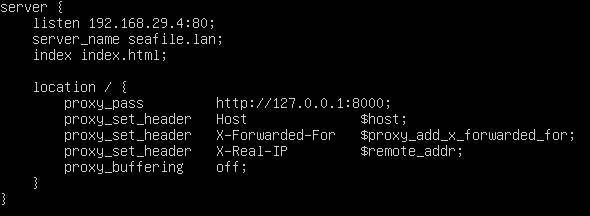
\includegraphics[width=0.85\textwidth]{img/08_nginx_conf}
  \caption{Конфигурация Nginx для обратного проксирования Seahub}
  \label{fig:nginx_conf}
\end{figure}

\section{Запуск Seafile и Seahub}

\begin{lstlisting}
/opt/seafile/seafile-server-9.0.9/seafile.sh start
/opt/seafile/seafile-server-9.0.9/seahub.sh start
\end{lstlisting}

При первом запуске \texttt{seahub.sh} предлагает создать учётную
запись администратора. Вводим e-mail в формате
\texttt{admin@STUDENT.GROUP.local} и пароль.

% — Скриншот: вывод seafile.sh start + seahub.sh start —
\begin{figure}[h]
  \centering
  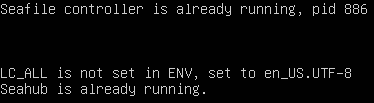
\includegraphics[width=0.85\textwidth]{img/09_seafile_start}
  \caption{Запуск сервисов Seafile и Seahub}
  \label{fig:seafile_start}
\end{figure}

\section{Настройка автозапуска}

Создаём systemd-unit для Seafile:
\begin{lstlisting}
nano /etc/systemd/system/seafile.service
\end{lstlisting}

Содержимое файла:
\begin{lstlisting}
[Unit]
Description=Seafile
After=mariadb.service
After=network.target

[Service]
Type=forking
ExecStart=/opt/seafile/seafile-server-9.0.9/seafile.sh start
ExecStop=/opt/seafile/seafile-server-9.0.9/seafile.sh stop

[Install]
WantedBy=multi-user.target
\end{lstlisting}

Активируем автозапуск и проверяем статус:
\begin{lstlisting}
systemctl enable seafile
systemctl enable seahub
systemctl status seafile
\end{lstlisting}

% — Скриншот: systemctl status seafile (active/running) —
\begin{figure}[h]
  \centering
  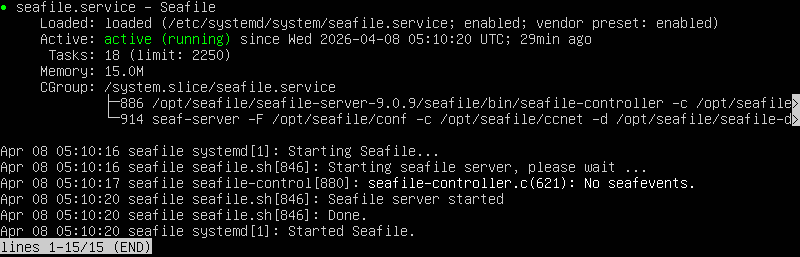
\includegraphics[width=0.85\textwidth]{img/11_seafile_service}
  \caption{Статус сервиса \texttt{seafile} — active (running)}
  \label{fig:seafile_service}
\end{figure}

\section{Проверка через веб-консоль}

На ВМ Desktop открываем браузер и переходим по адресу:
\begin{lstlisting}
http://seafile
\end{lstlisting}

Входим с учётной записью администратора\\
\texttt{admin@STUDENT.GROUP.local}.

% — Скриншот: страница входа Seafile в браузере —
\begin{figure}[h]
  \centering
  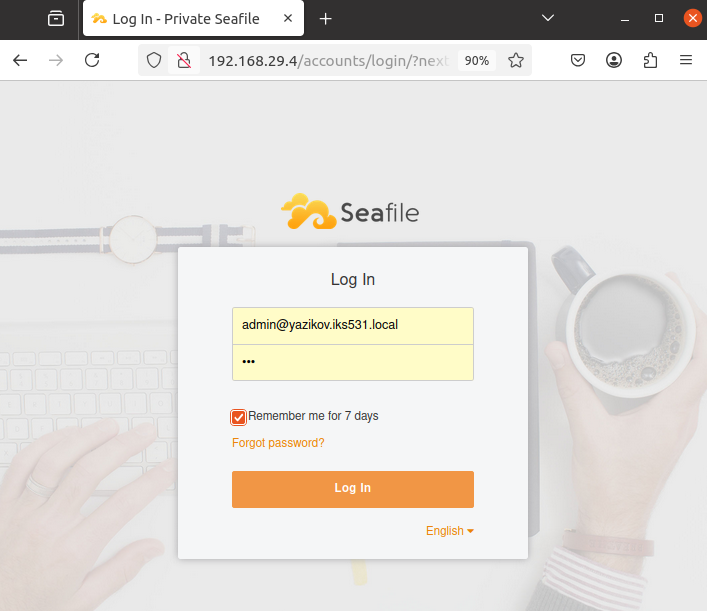
\includegraphics[width=0.85\textwidth]{img/12_seafile_web_login}
  \caption{Веб-интерфейс Seafile — страница входа}
  \label{fig:seafile_login}
\end{figure}

% — Скриншот: главная страница библиотек —
\begin{figure}[h]
  \centering
  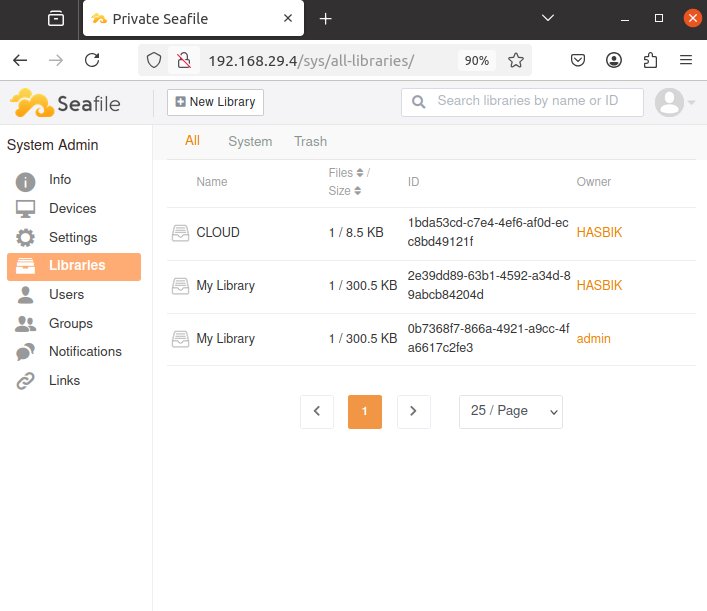
\includegraphics[width=0.85\textwidth]{img/13_seafile_web_library}
  \caption{Веб-интерфейс Seafile — библиотека с загруженным файлом}
  \label{fig:seafile_library}
\end{figure}

\section{Установка клиента Seafile на Desktop}

Выполняем на ВМ Desktop:
\begin{lstlisting}
sudo su
add-apt-repository ppa:seafile/seafile-client
apt-get update
apt-get install seafile-gui
\end{lstlisting}

\subsection{Синхронизация библиотеки}

Запускаем клиент, вводим адрес сервера \texttt{http://192.168.\cfgLabStudentN.4},
е-mail и пароль администратора, выбираем библиотеку и локальную папку для синхронизации.

% — Скриншот: клиент Seafile с синхронизированной библиотекой —
\begin{figure}[h]
  \centering
  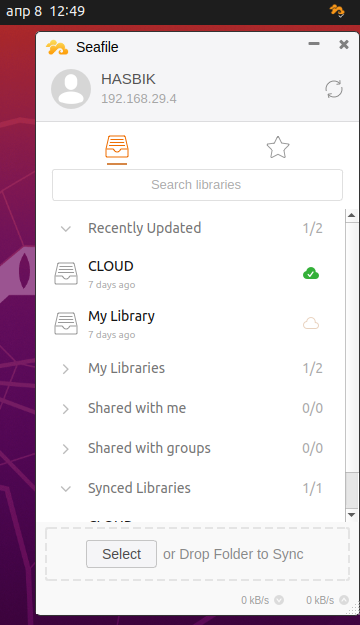
\includegraphics[width=0.85\textwidth]{img/15_seafile_client_sync}
  \caption{Клиент Seafile на Desktop — синхронизированная библиотека}
  \label{fig:seafile_sync}
\end{figure}

\endinput
